% 2003 年江苏卷第 22 题：直线与曲线迭代蛛网图
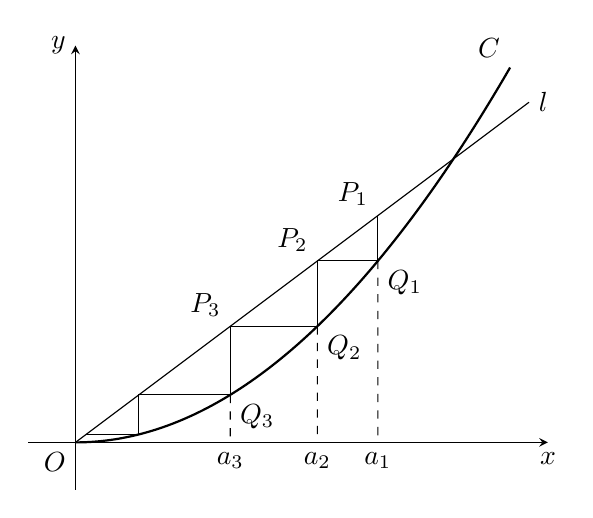
\begin{tikzpicture}[>=stealth,scale=1.2]
  % Parameters
  \def\slopeL{0.75}
  \def\cParab{0.1875} % 3.0 / 16.0
  
  \def\aOne{3.2}
  \def\aTwo{2.56}
  \def\aThree{1.6384}
  \def\aFour{0.671}
  
  % Coordinates of staircase
  \coordinate (P1) at (\aOne, {\slopeL*\aOne});
  \coordinate (Q1) at (\aOne, {\cParab*\aOne*\aOne});
  
  \coordinate (P2) at (\aTwo, {\cParab*\aOne*\aOne});
  \coordinate (Q2) at (\aTwo, {\cParab*\aTwo*\aTwo});
  
  \coordinate (P3) at (\aThree, {\cParab*\aTwo*\aTwo});
  \coordinate (Q3) at (\aThree, {\cParab*\aThree*\aThree});
  
  \coordinate (P4) at (\aFour, {\cParab*\aThree*\aThree});
  \coordinate (Q4) at (\aFour, {\cParab*\aFour*\aFour});
  \coordinate (P5) at ({\cParab*\aFour*\aFour / \slopeL}, {\cParab*\aFour*\aFour});
  
  % Axes
  \draw[->] (-0.5,0) -- (5.0,0) node[below] {$x$};
  \draw[->] (0,-0.5) -- (0,4.2) node[left] {$y$};
  \node[below left] at (0,0) {$O$};
  
  % Line l
  \draw (0,0) -- (4.8, {4.8*\slopeL}) node[right] {$l$};
  
  % Curve C
  \draw[thick, domain=0:4.6, samples=100] plot (\x, {\cParab*\x*\x}) node[above left] {$C$};
  
  % Staircase
  \draw (P1) -- (Q1) -- (P2) -- (Q2) -- (P3) -- (Q3) -- (P4) -- (Q4) -- (P5);
  
  % Dashed projections to x axis
  \draw[dashed] (Q1) -- (\aOne, 0) node[below] {$a_1$};
  \draw[dashed] (Q2) -- (\aTwo, 0) node[below] {$a_2$};
  \draw[dashed] (Q3) -- (\aThree, 0) node[below] {$a_3$};
  
  % Labels
  \node[above left] at (P1) {$P_1$};
  \node[above left] at (P2) {$P_2$};
  \node[above left] at (P3) {$P_3$};
  \node[below right] at (Q1) {$Q_1$};
  \node[below right] at (Q2) {$Q_2$};
  \node[below right] at (Q3) {$Q_3$};
\end{tikzpicture}
